%%%% Proceedings format for most of ACM conferences (with the exceptions listed below) and all ICPS volumes.
\documentclass[sigconf]{acmart}
%%%% As of March 2017, [siggraph] is no longer used. Please use sigconf (above) for SIGGRAPH conferences.

%%%% Proceedings format for SIGPLAN conferences 
% \documentclass[sigplan, anonymous, review]{acmart}

%%%% Proceedings format for SIGCHI conferences
% \documentclass[sigchi, review]{acmart}

%%%% To use the SIGCHI extended abstract template, please visit
% https://www.overleaf.com/read/zzzfqvkmrfzn


%%%%%%%%%%%%%%%%%%%%%%%%%%%%%%%%%%%%%%%%%%%%%%%%%%%%%%%%%%%%%%%%%%%%%%%%%%%%%%%%%%%%%%%%%%%%%%%%%%%%%%%%%%%%%%%%%%%%%%%%%%%%%%%%%%%%%%%%%%%%%%%%%%%%%%%%%
% PACKAGES
%%%%%%%%%%%%%%%%%%%%%%%%%%%%%%%%%%%%%%%%%%%%%%%%%%%%%%%%%%%%%%%%%%%%%%%%%%%%%%%%%%%%%%%%%%%%%%%%%%%%%%%%%%%%%%%%%%%%%%%%%%%%%%%%%%%%%%%%%%%%%%%%%%%%%%%%%
\usepackage{booktabs} % For formal tables
%% perso packages:
\usepackage{epstopdf}
\usepackage{microtype}
\usepackage{tabularx}
\usepackage{multirow}
%\usepackage{arydshln}
\usepackage{subfig}
\usepackage{balance}
\usepackage{caption}
\usepackage{graphicx}
\usepackage{amsmath}

%%%%%%%%%%%%%%%%%%%%%%%%%%%%%%%%%%%%%%%%%%%%%%%%%%%%%%%%%%%%%%%%%%%%%%%%%%%%%%%%%%%%%%%%%%%%%%%%%%%%%%%%%%%%%%%%%%%%%%%%%%%%%%%%%%%%%%%%%%%%%%%%%%%%%%%%%
% DOCUMENT's Identification
%%%%%%%%%%%%%%%%%%%%%%%%%%%%%%%%%%%%%%%%%%%%%%%%%%%%%%%%%%%%%%%%%%%%%%%%%%%%%%%%%%%%%%%%%%%%%%%%%%%%%%%%%%%%%%%%%%%%%%%%%%%%%%%%%%%%%%%%%%%%%%%%%%%%%%%%%
% Copyright
%\setcopyright{none}
%\setcopyright{acmcopyright}
%\setcopyright{acmlicensed}
\setcopyright{rightsretained}
%\setcopyright{usgov}
%\setcopyright{usgovmixed}
%\setcopyright{cagov}
%\setcopyright{cagovmixed}


% DOI
\acmDOI{10.475/123_4}

% ISBN
\acmISBN{123-4567-24-567/08/06}


%%%%%%%%%%%%%%%%%%%%%%%%%%%%%%%%%%%%%%%%%%%%%%%%%%%%%%%%%%%%%%%%%%%%%%%%%%%%%%%%%%%%%%%%%%%%%%%%%%%%%%%%%%%%%%%%%%%%%%%%%%%%%%%%%%%%%%%%%%%%%%%%%%%%%%%%%
% CONFERENCE
%%%%%%%%%%%%%%%%%%%%%%%%%%%%%%%%%%%%%%%%%%%%%%%%%%%%%%%%%%%%%%%%%%%%%%%%%%%%%%%%%%%%%%%%%%%%%%%%%%%%%%%%%%%%%%%%%%%%%%%%%%%%%%%%%%%%%%%%%%%%%%%%%%%%%%%%%
%Conference
\acmConference[ICMR 2018]{ACM Yokohama conference}{June 2018}{Yokohama, Japan} 
\acmYear{2018}
%\copyrightyear{2018}
%\acmArticle{4}%??
%\acmPrice{15.00}%??

%%%%%%%%%%%%%%%%%%%%%%%%%%%%%%%%%%%%%%%%%%%%%%%%%%%%%%%%%%%%%%%%%%%%%%%%%%%%%%%%%%%%%%%%%%%%%%%%%%%%%%%%%%%%%%%%%%%%%%%%%%%%%%%%%%%%%%%%%%%%%%%%%%%%%%%%%
\begin{document}
%%%%%%%%%%%%%%%%%%%%%%%%%%%%%%%%%%%%%%%%%%%%%%%%%%%%%%%%%%%%%%%%%%%%%%%%%%%%%%%%%%%%%%%%%%%%%%%%%%%%%%%%%%%%%%%%%%%%%%%%%%%%%%%%%%%%%%%%%%%%%%%%%%%%%%%%%

%%%%%%%%%%%%%%%%%%%%%%%%%%%%%%%%%%%%%%%%%%%%%%%%%%%%%%%%%%%%%%%%%%%%%%%%%%%%%%%%%%%%%%%%%%%%%%%%%%%%%%%%%%%%%%%%%%%%%%%%%%%%%%%%%%%%%%%%%%%%%%%%%%%%%%%%%
% TITLE
%%%%%%%%%%%%%%%%%%%%%%%%%%%%%%%%%%%%%%%%%%%%%%%%%%%%%%%%%%%%%%%%%%%%%%%%%%%%%%%%%%%%%%%%%%%%%%%%%%%%%%%%%%%%%%%%%%%%%%%%%%%%%%%%%%%%%%%%%%%%%%%%%%%%%%%%%
\title{Annotating, understanding, and predicting long-term video memorability}
%\titlenote{}
%\subtitle{}
%\subtitlenote{}

%%%%%%%%%%%%%%%%%%%%%%%%%%%%%%%%%%%%%%%%%%%%%%%%%%%%%%%%%%%%%%%%%%%%%%%%%%%%%%%%%%%%%%%%%%%%%%%%%%%%%%%%%%%%%%%%%%%%%%%%%%%%%%%%%%%%%%%%%%%%%%%%%%%%%%%%%
% AUTHORS
%%%%%%%%%%%%%%%%%%%%%%%%%%%%%%%%%%%%%%%%%%%%%%%%%%%%%%%%%%%%%%%%%%%%%%%%%%%%%%%%%%%%%%%%%%%%%%%%%%%%%%%%%%%%%%%%%%%%%%%%%%%%%%%%%%%%%%%%%%%%%%%%%%%%%%%%%
%author 1
%\author{Romain Cohendet}
%\authornote{}
%\orcid{1234-5678-9012}
%\affiliation{%
%	\institution{Technicolor}
%	\streetaddress{Technicolor Research \& Licensing, 975 Avenue des Champs Blancs, 35576 Cesson-Sevigne, France}
%	\city{Rennes} 
%	\state{France} 
%	\postcode{}
%}
%\email{romain.cohendet@technicolor.com}

%author 2
%\author{Karthik Yadati}
%\affiliation{%
%	\institution{University of Delft}
%	\streetaddress{}
%	\city{Delft} 
%	\state{} 
%	\postcode{}
%}
%\email{N.K.Yadati@tudelft.nl}

%author 3
%\author{Ngoc Khanh Duong}
%\affiliation{%
%	\institution{Technicolor}
%	\city{Rennes} 
%	\country{France}}
%\email{Quang-Khanh-Ngoc.Duong@technicolor.com}

%author 4
%\author{Claire-Helene Demarty}
%\affiliation{%
%	\institution{Technicolor}
%	\city{Rennes}
%	\country{France}
%}
%\email{Claire-Helene.Demarty@technicolor.com}

%%%%%%%%%%%%
%%% for blind review %%%
%author 1
%\author{Removed for review}
%author 2
%\author{Removed for review}

% The default list of authors is too long for headers.
\renewcommand{\shortauthors}{Removed for blind review}%{R. Cohendet et al.}%Removed for blind review

%%%%%%%%%%%%%%%%%%%%%%%%%%%%%%%%%%%%%%%%%%%%%%%%%%%%%%%%%%%%%%%%%%%%%%%%%%%%%%%%%%%%%%%%%%%%%%%%%%%%%%%%%%%%%%%%%%%%%%%%%%%%%%%%%%%%%%%%%%%%%%%%%%%%%%%%%
% ABSTRACT
%%%%%%%%%%%%%%%%%%%%%%%%%%%%%%%%%%%%%%%%%%%%%%%%%%%%%%%%%%%%%%%%%%%%%%%%%%%%%%%%%%%%%%%%%%%%%%%%%%%%%%%%%%%%%%%%%%%%%%%%%%%%%%%%%%%%%%%%%%%%%%%%%%%%%%%%%
\begin{abstract}
%The growing number of video contents on the Internet encourages us to find new ways to make more relevant their occurrences in our everyday life.
Memorability can be regarded as a useful metric of video importance to help make a choice between competing videos.
Research on computational understanding of video memorability is however in its early stages.
There is no available dataset for modelling purposes, and the few previous attempts provided protocols to collect video memorability data that would be difficult to generalize.
Furthermore, the computational features needed to build a robust memorability predictor remain largely undiscovered.
In this article, we propose a new protocol to collect long-term video memorability annotations.
We measure the memory performances of 104 participants from weeks to years after memorization to build a dataset of 660 videos for video memorability prediction.
This dataset is made available for the research community.
We then analyze the collected data in order to better understand video memorability, in particular the effects of response time, duration of memory retention and repetition of visualization on video memorability.
We finally investigate the use of various types of audio and visual features and build a computational model for video memorability prediction. We conclude that high level visual semantics help better predict the memorability of videos. 
\end{abstract}

%%%%%%%%%%%%%%%%%%%%%%%%%%%%%%%%%%%%%%%%%%%%%%%%%%%%%%%%%%%%%%%%%%%%%%%%%%%%%%%%%%%%%%%%%%%%%%%%%%%%%%%%%%%%%%%%%%%%%%%%%%%%%%%%%%%%%%%%%%%%%%%%%%%%%%%%%
%% NEW ACM TAXONOMY to categorise ACM article
%%%%%%%%%%%%%%%%%%%%%%%%%%%%%%%%%%%%%%%%%%%%%%%%%%%%%%%%%%%%%%%%%%%%%%%%%%%%%%%%%%%%%%%%%%%%%%%%%%%%%%%%%%%%%%%%%%%%%%%%%%%%%%%%%%%%%%%%%%%%%%%%%%%%%%%%%
\begin{CCSXML}
	<ccs2012>
	<concept>
	<concept_id>10010520.10010553.10010562</concept_id>
	<concept_desc>Computer systems organization~Embedded systems</concept_desc>
	<concept_significance>500</concept_significance>
	</concept>
	<concept>
	<concept_id>10010520.10010575.10010755</concept_id>
	<concept_desc>Computer systems organization~Redundancy</concept_desc>
	<concept_significance>300</concept_significance>
	</concept>
	<concept>
	<concept_id>10010520.10010553.10010554</concept_id>
	<concept_desc>Computer systems organization~Robotics</concept_desc>
	<concept_significance>100</concept_significance>
	</concept>
	<concept>
	<concept_id>10003033.10003083.10003095</concept_id>
	<concept_desc>Networks~Network reliability</concept_desc>
	<concept_significance>100</concept_significance>
	</concept>
	</ccs2012>  
\end{CCSXML}

%\ccsdesc[500]{Computer systems organization~Embedded systems}
%\ccsdesc[300]{Computer systems organization~Redundancy}
%\ccsdesc{Computer systems organization~Robotics}
%\ccsdesc[100]{Networks~Network reliability}

%%%%%%%%%%%%%%%%%%%%%%%%%%%%%%%%%%%%%%%%%%%%%%%%%%%%%%%%%%%%%%%%%%%%%%%%%%%%%%%%%%%%%%%%%%%%%%%%%%%%%%%%%%%%%%%%%%%%%%%%%%%%%%%%%%%%%%%%%%%%%%%%%%%%%%%%%
% KEYWORDS
%%%%%%%%%%%%%%%%%%%%%%%%%%%%%%%%%%%%%%%%%%%%%%%%%%%%%%%%%%%%%%%%%%%%%%%%%%%%%%%%%%%%%%%%%%%%%%%%%%%%%%%%%%%%%%%%%%%%%%%%%%%%%%%%%%%%%%%%%%%%%%%%%%%%%%%%%
\keywords{Video memorability, Long-term memory, Measurement protocol, Deep learning, Multimedia information retrieval}

%%%%%%%%%%%%%%%%%%%%%%%%%%%%%%%%%%%%%%%%%%%%%%%%%%%%%%%%%%%%%%%%%%%%%%%%%%%%%%%%%%%%%%%%%%%%%%%%%%%%%%%%%%%%%%%%%%%%%%%%%%%%%%%%%%%%%%%%%%%%%%%%%%%%%%%%%
%% ABOUT ICMR'2018 article...
%%%%%%%%%%%%%%%%%%%%%%%%%%%%%%%%%%%%%%%%%%%%%%%%%%%%%%%%%%%%%%%%%%%%%%%%%%%%%%%%%%%%%%%%%%%%%%%%%%%%%%%%%%%%%%%%%%%%%%%%%%%%%%%%%%%%%%%%%%%%%%%%%%%%%%%%%
\maketitle
%if we want the text be called from there
 %\input{samplebody-conf}

%% About the ICMR article on Media retrieval with VM
	% focus on "Multimedia content-based retrieval"
	% Length: from 6 to 8 pages + 1 additional page for references (no longer distinction between long and short papers)
	% Submission deadline: 2018/01/20
	% Contributions addressing the challenges of large-scale search and user behavior analysis are especially welcome

%%%%%%%%%%%%%%%%%%%%%%%%%%%%%%%%%%%%%%%%%%%%%%%%%%%%%%%%%%%%%%%%%%%%%%%%%%%%%%%%%%%%%%%%%%%%%%%%%%%%%%%%%%%%%%%%%%%%%%%%%%%%%%%%%%%%%%%%%%%%%%%%%%%%%%%%%
\section{Introduction}%nb of sections %2 PAGES
%%%%%%%%%%%%%%%%%%%%%%%%%%%%%%%%%%%%%%%%%%%%%%%%%%%%%%%%%%%%%%%%%%%%%%%%%%%%%%%%%%%%%%%%%%%%%%%%%%%%%%%%%%%%%%%%%%%%%%%%%%%%%%%%%%%%%%%%%%%%%%%%%%%%%%%%%
%opening
Enhancing the relevance of multimedia occurrences in our everyday life requires new ways to organize -- in particular, to retrieve -- digital content.
Like other metrics of video "importance", such as aesthetics \cite{dhar_2011_high} or interestingness \cite{demarty_2016_mediaeval}, memorability can be regarded as useful to help make a choice between competing videos.
In addition, memorability has the advantage of being clearly definable and objectively measurable (i.e., using a measure that is not influenced by the observer's personal judgment).
Image memorability has initially been defined as the probability for an image to be recognized \textbf{a few minutes} after a single view, when presented amidst a stream
of images \cite{isola_2011_makes}.
This definition has been widely accepted within subsequent work (e.g., \cite{mancas_2013_memorability,kim_2013_relative,celikkale_2013_visual,khosla_2015_understanding,lahrache_2016_bag}).

%from images to VM
The computational understanding of video memorability (VM) follows on from the study of image memorability (IM) prediction which has attracted increasing attention since the seminal work of Isola \textit{et al.} \cite{isola_2011_makes}.
With the recent introduction of deep learning to address the challenge of IM prediction, models also achieved very good results \cite{khosla_2015_understanding,baveye_2016_deep,squalli_2017_deep}.
As a result of this success, researchers have recently extended this challenge to videos.
However, to the best of our knowledge, only two available studies focus on VM prediction \cite{han_2015_learning,shekhar_2017_show}.

%explain the scarcity of studies on VM
Several problems could explain this scarcity of studies on VM.
Firstly, there is no publicly available dataset to train and test models.
This is probably the most serious obstacle to the rapid expansion of research in VM prediction.
Following the foot steps of researchers in IM \cite{isola_2011_makes,khosla_2015_understanding}, providing data and ground truth for VM should be one of our first objectives.
The second point, closely related to the previous one, is the lack of a common definition for VM.
The previous attempts to predict VM \cite{han_2015_learning,shekhar_2017_show} were based on different measures of memorability.
Furthermore, in comparison to images, videos have supplementary dimensions -- sound and visual movement -- that critically contribute to the semantic and emotional information conveyed and this makes it difficult to come up with a common definition of VM.
But the videos used and the way memorability is measured have a critical impact on what we understand by VM.
Similarly, the definition of IM \cite{isola_2011_makes} inevitably limited researchers.
In particular, previous research on IM focused on the measurement of memory performances only a few minutes after memorization.
But these short-term memory performances might be poor predictors of longer term memory performances.
For example, the memorability of emotional images would decrease in a non-harmonious way between two measures of memory performance (a few minutes and one day after memorization), inducing in a dataset a change in the ranking of memorability values over time \cite{cohendet_2016_prediction}.
To this end, VM data would be expected to benefit from a protocol that would measure lasting long-term memory performance.

%modelling
Regarding modelling, the previous attempts at predicting VM \cite{han_2015_learning,shekhar_2017_show} highlighted several features which contribute to the prediction of VM, such as semantic, saliency and color features.
But the work is far from complete and our capacity to propose efficient computational models will participate to answer the challenge of VM prediction.

%objectives of the present study
While participating in the expansion of research on VM, the contributions of this paper are threefold:
\begin{itemize}
	\item We propose a new protocol that measures very long-term memory performances (from weeks to years after memorization) to collect ground truth data of good quality and make the corresponding dataset available for the research community (section \ref{section_dataset_construction}).
	\item We assess and analyze the collected data and provide useful insights on the understanding of VM (section \ref{study_memorability}).
	\item We build a computational model based on machine learning techniques which allows to predict VM score of a given video. For this purpose, we investigate the use of various types of audio and visual features, ranging from low-level characteristics to emotional and (highly) semantic features (section \ref{mem-pred}).
\end{itemize}

%%%%%%%%%%%%%%%%%%%%%%%%%%%%%%%%%%%%%%%%%%%%%%%%%%%%%%%%%%%%%%%%%%%%%%%%%%%%%%%%%%%%%%%%%%%%%%%%%%%%%%%%%%%%%%%%%%%%%%%%%%%%%%%%%%%%%%%%%%%%%%%%%%%%%%%%%
\section{Previous work}
In this section, we review previous work on image and video memorability prediction, focusing on annotation protocols and modelling aspects.
%%%%%%%%%%%%%%%%%%%%%%%%%%%%%%%%%%%%%%%%%%%%%%%%%%%%%%%%%%%%%%%%%%%%%%%%%%%%%%%%%%%%%%%%%%%%%%%%%%%%%%%%%%%%%%%%%%%%%%%%%%%%%%%%%%%%%%%%%%%%%%%%%%%%%%%%%
\subsection{Measurement of memorability}
%work in psychology
Long-term memory has been studied for over a century in psychology, from multiple perspectives, since the seminal experimental studies of Ebbinghaus \cite{ebbinghaus_1913_memory} until the more recent neuro-imaging studies \cite{blumenfeld_2007_prefrontal}.
This work provided researchers, interested in computational understanding of IM and VM, with several memory tests (see \cite{richardson_1988_measures} for an extensive overview), such as the recognition test \cite{isola_2011_makes,khosla_2015_understanding,han_2015_learning} or the textual questions-based recall survey \cite{shekhar_2017_show}.
It also demonstrated that humans have an extensive long-term visual memory, which enables them to recall a great amount of images \cite{standing_1973_learning} and image details \cite{brady_2008_visual}, as well as of videos \cite{furman_2007_they}.
This is one of the observations at the origin of the work on memorability in computer science \cite{isola_2011_makes}.
Several factors have also been highlighted for their critical influence on long-term memory, such as emotion \cite{kensinger_2008_memory}, semantics \cite{quillan_1966_semantic}, several demographic factors \cite{cohendet_2016_using}, memory re-evocation \cite{nadel_1997_memory}, or passage of time \cite{mcgaugh_2000_memory}.
These different factors are all important to better understand memorability, and are found valuable computational features for image and video memorability prediction.

%Images work -- towards a long-term memorability
Focusing on the work in computer vision, most studies on IM prediction made use of one of the two available large datasets designed specifically to meet this challenge \cite{isola_2011_makes,khosla_2015_understanding}.
To address more specific problems, several other datasets have also been publicly released concerning memorability of face photographs \cite{bainbridge_2013_intrinsic}, visualization pictures \cite{borkin_2013_makes}, emotional images \cite{cohendet_2016_using} and scene categories \cite{bylinskii_2015_intrinsic}.
To build the most used datasets presented in \cite{isola_2011_makes,khosla_2015_understanding}, the authors, possibly constrained by the difficulty in conducting long crowdsourcing studies, measured memory performance a few minutes after memorization to obtain their memorability annotations.
This could be a problem if we conceive that memorability reflects a lasting memory performance \cite{cohendet_2016_prediction}.
Indeed, it has been shown that long-term memories continue to change long after their memorization through an ongoing process called consolidation, which lasts weeks to years \cite{mcgaugh_2000_memory}.
%In particular, the early work of the psychologist Ebbinghaus showed that the drop in long-term memory performance in recall follow an exponential decay, and is particularly strong in the few days immediately following the memorization \cite{ebbinghaus_1913_memory}.
Because several factors influence the consolidation process (e.g., emotions, sleep, re-evocation), which does not equally affect all memories, the order of memorability ratings measured for content, and especially videos, is susceptible to change over time \cite{cohendet_2016_prediction}.
A protocol to collect memorability annotations would benefit from the capacity to capture long-lasting memory performances, averaged to obtain what we will later refer to as "long-term memorability".

%Han et al.
To our knowledge, the first attempt at measuring VM \cite{han_2015_learning} partially adapted the protocol proposed to measure IM \cite{isola_2011_makes} to videos.
The resulting protocol is however much heavier than the memory game protocol \cite{isola_2011_makes}.
They followed a classical recognition process, which consists of two steps: a free viewing task, followed two days later by a recall task.
The task duration, for each of the 20 participants, was about 24 hours, spread over 10 sessions (five free viewing tasks and five recall tasks) of about two hours each.
The authors used the same proportion of fillers (i.e., non repeated videos) in the free viewing and recall tasks (i.e., 4/5 of fillers and 1/5 of repeated videos named targets) to guarantee that viewers were unaware of targets.
If it was mandatory in \cite{isola_2011_makes} for which encoding and recall tasks were interlaced, there is a way here to alleviate the task without impacting its quality; indeed, reducing the number of fillers in the free viewing task would have very little impact on the memorability scores (often authors even use only material interrogated later in the learning/free viewing task).
Furthermore, the long time span of the experiment makes the generalization of this protocol difficult, in particular if one targets the construction of an extensive dataset.
Moreover, authors measured memory after two days, but, as aforementioned, it is known that the consolidation process lasts weeks to years: it would be interesting to collect even longer term memory performances.

%Shekhar et al.
In another earlier approach for VM measurement, the participants performed a crowdsourcing experiment that consisted of a free viewing task during which they saw a series of videos, followed by a recall task in which they had to answer textual questions (such as: "Did you see a man juggling?", "Did you see a car on road?") \cite{shekhar_2017_show}.
The major drawback of the study comes from the use of questions instead of a classic visual recognition task.
Indeed, the memorability scores computed for the videos may reflect not only the differences in memory performances but also the differences between the questions in terms of difficulty.
The authors tested the complexity of the chosen textual questions using the Flesch-Kincaid Grade Level readability metric, which is designed to quantify how difficult to understand an English text is \cite{kincaid_1975_derivation}.
However, this measure might not be sufficient to represent the questions in all their complexities, such as the ease for a person to draw images from the words, to connect the words to the associated concepts in memory, to associate the words to the corresponding scene, etc.
Moreover, there is an unequal distribution of the reading comprehension of English among Amazon Mechanical Turk workers, who are not necessary anglophone people.
This problem of a potential unequal complexity of the question becomes even more important in view of the use by authors of the response time to calculate memorability scores, which might also critically depend on the complexity of the questions.
One will note that this potential bias could have also affected the measure of inter-human consistency.
Furthermore, the questions were handcrafted, and the choices for types of questions and videos were very limited (e.g., the question "Did you see a car on road?" implies that in a whole experimental session only one car on a road should appear to connect the memory performance to one particular video).
The authors also manually ensured that no textual questions nor videos in a session were similar in content.
This makes it difficult to generalize this protocol to the construction of an extensive dataset.

\subsection{Memorability modelling}
%intro on focus on features to discover
Previous attempts at predicting image and video memorability highlighted quite a few features that correlate with memorability.

%IM prediction
The pioneering work of Isola \textit{et al.} focused primarily on building computational models to predict IM from low-level visual features \cite{isola_2011_makes}.
From their work, it appeared that the degree of an image's memorability can be predicted to a certain extent.
Several characteristics have also been found to be relevant for predicting memorability in subsequent work, for example saliency \cite{mancas_2013_memorability}, interestingness and aesthetics \cite{isola_2014_makes}, or emotions \cite{khosla_2015_understanding}.
The best results were finally obtained by using fine-tuned deep features, which outperformed all other features in \cite{khosla_2015_understanding}, reaching a rank correlation of $.64$ which is near human consistency ($.68$) when measured for the ground truth collected in the study.
This result was later confirmed by other researchers \cite{baveye_2016_deep,squalli_2017_deep}.

%VM prediction
Regarding VM prediction, Han \textit{et al.} proposed a method which combines the power of audio-visual and fMRI-derived features \cite{han_2015_learning}.
They preliminary built a computational model learned with fMRI features, which supposedly conveys the brain activity of memorizing videos.
This enabled them to finally predict VM without the use of fMRI scans in a second step.
However, the method would be difficult to generalize.
Shekhar \textit{et al.} conducted a performance analysis of several computationally extracted features before building their memorability predictor \cite{shekhar_2017_show}.
The analysis encompassed C3D deep learning features, semantic features obtained from some video captioning process, saliency features, dense trajectories, and color features.
They found that the most predictive feature combination used captioning features, dense trajectories, saliency and color features.
The features that performed the best when used alone were image captioning features, i.e., those conveying more semantics.
Due to the particularity of the dataset of Shekhar \textit{et al.} -- that is, their aforementioned use of questions to measure memorability --, it would be interesting to confirm if this combination works equally well on another dataset, and in particular if image captioning features also perform the best.

%%%%%%%%%%%%%%%%%%%%%%%%%%%%%%%%%%%%%%%%%%%%%%%%%%%%%%%%%%%%%%%%%%%%%%%%%%%%%%%%%%%%%%%%%%%%%%%%%%%%%%%%%%%%%%%%%%%%%%%%%%%%%%%%%%%%%%%%%%%%%%%%%%%%%%%%%
\section{Memorability dataset construction}
\label{section_dataset_construction}
%%%%%%%%%%%%%%%%%%%%%%%%%%%%%%%%%%%%%%%%%%%%%%%%%%%%%%%%%%%%%%%%%%%%%%%%%%%%%%%%%%%%%%%%%%%%%%%%%%%%%%%%%%%%%%%%%%%%%%%%%%%%%%%%%%%%%%%%%%%%%%%%%%%%%%%%%
\subsection{Video collection}
%why did we choose movies
We want our protocol to measure memory performance after a significant retention period.
This can be achieved either with a longitudinal study, or by measuring a memory created prior to the experiment.
We chose the latter because it enabled us to immediately measure very long-term memory.
Thus, the main characteristic of the proposed protocol, in contrast with previous work, is the absence of learning (often, free viewing) task.
It is replaced with a questionnaire designed to collect information about the participants' prior memory.
In order to repeat measures of memory performances for different persons on the same material, to obtain average performance, we worked with movies famous enough to have been seen by several of our participants.

%movies and videos selections
 %with HD or dvdrip quality, in orginal (i.e.,english) version, without without subtitles [add if results HD vs. DVDrip]
 %sauf slumdog millionaire
We first established a list of 100 occidental movies, taking care of mixing popularity and genres.
We then manually selected seven videos of 10 seconds from each movie.
To maintain a high intra-video semantic cohesion, we did not make cuts that would impair the understanding of the scene, nor did we aggregate shots that belong to different scenes.
Indeed, since the semantics is linked to the memorability of images \cite{isola_2014_makes}, we can expect it is linked to the memorability of videos too.

%neutral vs. typical
We also gave preference to the videos we called "neutral", by contrast to the "typical" ones.
According to our definition, a neutral video is a part of a movie which contains no element that would enable someone to easily guess this video belongs to a particular movie.
The list of undesirable elements includes but is not limited to: recognizable famous actors, typical music, style, etc.
Typical videos are simply defined as non-neutral videos.
In most movies, just a few or no 10-second neutral videos exist.
That explains why we obtained only 127 neutral videos for 573 typical ones (while we expected two neutral and five typical videos per movie, i.e., 200 neutral and 500 typical videos in total).
 
%%%%%%%%%%%%%%%%%%%%%%%%
\subsection{Annotation protocol}
%presentation protocol
The protocol is composed of two tasks.
Firstly, participants had to fill in a questionnaire intended to collect data about whether they have seen the 100 selected movies.
Secondly, participants performed a recognition task on videos selected based on their responses to the questionnaire.

%participants, facilities and apparatus
104 participants ($22-58$ years of age; age average = 37.1; stdev = 10.4; $26\%$ females; mostly educated persons -- engineers or researchers mainly), participated in the experiment on a voluntary basis.
The experiment was taking place in a well-controlled environment: a room insulated from noise and equipped with subdued lights.
The videos, of HD or DVD quality, were displayed on a 60 inch monitor.
The participants were seated at a distance of about 220 centimeters from the screen (three times the screen height).
%questionnaire
 %Each item included a movie poster with its name below, followed by the question.
Having provided basic demographics, participants answered the questionnaire.
For each of the 100 movies, they were asked whether they remembered watching fully the movie.
In case of a positive answer, three additional questions followed: 1/ their confidence of watching the movie (\textit{not confident / slightly confident / 50\% confident / considerably confident / 100\% confident}), 2/ the last time they saw the movie (\textit{less than month / 1 year / 5 years / 10 years / more than 10 years}), and 3/ the number of times they saw the movie (\textit{once / 2-4 times / 5-9 times / 10-19 times / more than 20 times}).
In case of a negative answer, only one question was asked, related to their confidence of not having seen the movie.
The questionnaire required about 20 minutes to complete.

%Algorithm selection
Based on the answers to the questionnaire, an algorithm automatically selected 80 targets (i.e., videos from seen movies) and 40 fillers (i.e., videos from never seen movies) among the movies associated with the highest degree of certitude, with a maximum of two videos from the same movie.
The fillers enable to quantify how much lucky confusions account for the correct recognitions.
During the video selection, the current number of annotations was also taken into account to equally balance the annotations among all the videos.
%Recognition task
Given such 120 videos selected, participants performed a recognition task where they saw the videos separated by an inter-stimuli interval of 2 seconds.
They had to press the space bar when they recognized a video in particular, and not when they were guessing that a particular video came from a movie they had seen (which was possible only for the typical videos).
%In case a participant pressed the space bar, the video continued until its end.

%%%%%%%%%%%%%%%%%%%%%%%%
\subsection{Memorability score calculation}
%Each video has also been viewed as a filler by $10.5$ participants.
After collecting the data, we kept only the 660 videos that had been seen at least 4 times as targets (from the initial set of 700 videos).
On average, each video of our dataset has been viewed as a target by $10.7$ participants; which corresponds to the mean number of observations that enters in the calculation of a memorability score.
We then assigned a memorability score to each video, defined as the correct recognition rate of the video when viewed as target.
The average percentage of correct detections for all participants was $46.71\%$ (stdev = 14.65\%), and the average false alarm rate (i.e., the percentage of answers on fillers) was $4.16\%$ (stdev = 5.27\%).
Figure \ref{fig:response_time_vs_memorability}(a) provides a distribution of the videos according to their degree of memorability.
The dataset is publicly released here\footnote{\textit{www.remove-for-blind-review}. The original videos are not released because of copyright issues, but instead we provide the process we used to extract them from the movies and the features used in section \ref{mem-pred}.}.

%%%%%%%%%%%%%%%%%%%%%%%%%%%%%%%%%%%%%%%%%%%%%%%%%%%%%%%%%%%%%%%%%%%%%%%%%%%%%%%%%%%%%%%%%%%%%%%%%%%%%%%%%%%%%%%%%%%%%%%%%%%%%%%%%%%%%%%%%%%%%%%%%%%%%%%%%
\section{Study of the memorability annotations}
\label{study_memorability}
%%%%%%%%%%%%%%%%%%%%%%%%%%%%%%%%%%%%%%%%%%%%%%%%%%%%%%%%%%%%%%%%%%%%%%%%%%%%%%%%%%%%%%%%%%%%%%%%%%%%%%%%%%%%%%%%%%%%%%%%%%%%%%%%%%%%%%%%%%%%%%%%%%%%%%%%%
In this section, we conduct an analysis of the ground truth data collected through the protocol described above.
We firstly perform a human consistency analysis.
Then we compare neutral videos with typical videos.
We finally study which factors affect the memorability among response time, duration of memory retention and repetition of visualization.
In what follows, error bars in the graphs correspond to standard error of the mean, $\mu$ to the mean, $Mdn$ to the median and $N$ to the number of observations in the statistics.

%%%%%%%%%%%%%%%%%%%%%%%%
\subsection{Consistency analysis}
\label{ssec:human}
%global consistency calculation
We follow the method proposed in \cite{isola_2014_makes} to measure human consistency when assessing memorability of videos.
We randomly split our 104 participants into two independent groups of equal size, and calculate how well video memorability scores from the first group of participants match with video memorability scores from the second group.
Averaging over 25 random half-split trials, an average Spearman's rank correlation (i.e., a global human consistency) of $0.57$ is observed between these pairs of scores.

%Fig Consistency
 %Histogram of number of nb of videos per possibble nb of annotations
 %Graph of human consistency
\begin{figure}[!htbp]
	\centering
	\subfloat[]{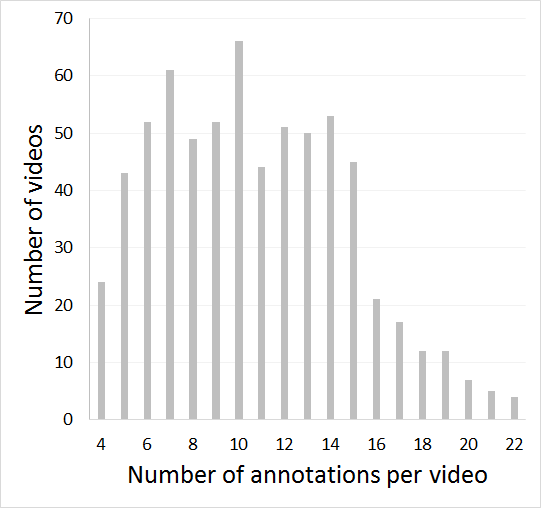
\includegraphics[width=0.45\columnwidth]{figures/histogram_nb_sequences_for_nb_of_annotations.png}}
	\quad
	\subfloat[]{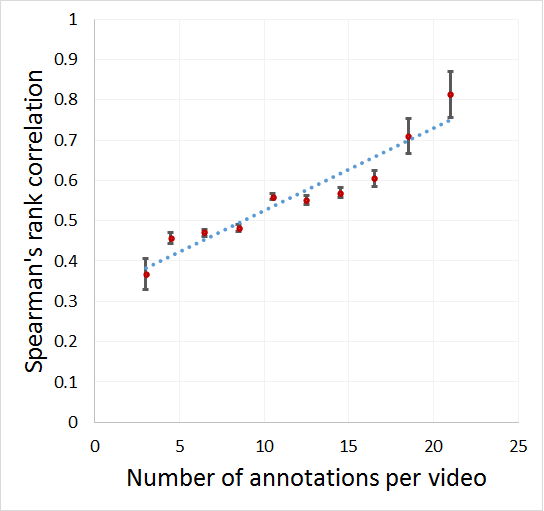
\includegraphics[width=0.45\columnwidth]{figures/Measure_of_human_consistency.png}}
	\quad
	\caption{\label{fig:human_consistency}(a) Distribution of the number of videos according to the number of annotations per video. (b) Human consistency (with linear trendline).}
\end{figure}

%per nb of annotations consistency %comparison with IM
We reproduced this calculation to obtain human consistency as a function of the number of annotations per video, presented in Figure \ref{fig:human_consistency}(b).
This graph is to be compared with the histogram presented in Figure \ref{fig:human_consistency}(a), which shows that the number of videos for each number of annotations was unequal.
According to the graph, we achieved a consistency of $.70$ from about 18 annotations, which is consistent with the previous finding \cite{han_2015_learning}.
This number also corresponds to the maximal consistency obtained when collecting IM scores \cite{isola_2011_makes,khosla_2015_understanding}, but for a much bigger number of annotations (80) per image.
It must be noted that the protocols are different between the IM experiments conducted in \cite{isola_2011_makes,khosla_2015_understanding} and ours or the work in \cite{han_2015_learning}.
We conducted a measure of long-term memory performance after at least two days of memorization, whereas in \cite{isola_2011_makes,khosla_2015_understanding} it is measured after a dozen of seconds to a few minutes. 
In addition, VM annotations were collected through in-lab experiments, and IM annotations through crowdsourcing experiments.
%These factors might have contributed to the smaller number of annotations necessary to reach a high human consistency for videos.
However, it would be interesting in the future to confirm if an important difference exists between images and videos regarding the number of annotations necessary to achieve a high human consistency.
Apart from the conclusions we could draw about the universality of the intrinsic memorability of videos compared to images, this would mean that the magnitude of the work to carry out to build an extensive database for VM prediction is substantially smaller than one could expect from work on IM prediction.

%%%%%%%%%%%%%%%%%%%%%%%%%%%%%%%%%%%%%
\subsection{Neutral and typical videos}
In our experiment, participants were given clear instructions that they had to really recognize any video they were presented as already seen, and not only guess that a video was coming from a movie whose title was proposed in the questionnaire.
In this section, we perform an analysis to compare neutral videos, which contain no element that would enable participants to guess that a video belongs to a particular movie, and typical videos.
Indeed, if neutral videos received objective answers from participants, it might be more subjective for typical videos, that could be more or less easily related to the movie they belong to.

A Wilcoxon rank-sum test indicated that the memorability was greater for neutral ($Mdn=.20, \mu=.24$) than for typical ($Mdn=.53, \mu=.53$) videos, with $Z=10.22, p<.00001$.
Apart from the subjectivity aspect, we expected such a result because neutral videos contain less contextual elements, useful for recognition.
Thus, this result does not necessarily mean that participants tended to guess -- rather than simply recognize -- videos selected from movies they have seen.

As for the human consistency on memorability, a Wilcoxon rank-sum test indicated that it was slightly greater for neutral ($Mdn=.44, \mu=.45$) than for typical ($Mdn=.40, \mu=.41$) videos, with $Z=2.75, p<.01$.
Along with the comments collected from the participants, who have as a majority reported difficulty to know if they were guessing or really recognizing the videos, this result suggests that human congruency is higher for more 'objectively' recognized segments than for ones with subjectivity as part of the equation. 
One could note there is probably not just pure subjectivity here.
Context might have biased the results as it might have helped some participants in their recognition task.
If confirmed, this would constitute a weakness of our protocol to collect extensive data, that one should in that case counteract by adapted measures of control.

We can also note that the average false alarm rate (that is, the percentage of wrongly recognized filler videos) was low for neutral videos ($.05\%$) as well as for typical videos ($.03\%$).
Specifically, we expect lucky confusions to account for little of correct detections on average for the two sorts of videos.

%%%%%%%%%%%%%%%%%%%%%%%%%%%%%%%%%%%%%
\subsection{Response time}
%figure Distribution of memorability scores + Mean response time vs. degrees of memorability
\begin{figure}[!htbp]
	\centering
	\subfloat[]{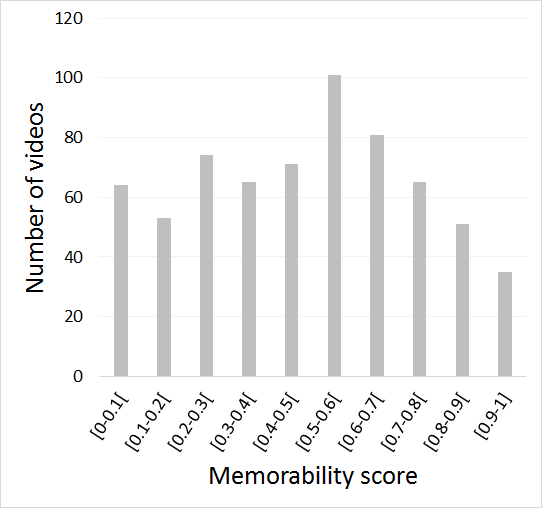
\includegraphics[width=0.45\columnwidth]{figures/memorability_scores_distribution.png}}
	\quad
	\subfloat[]{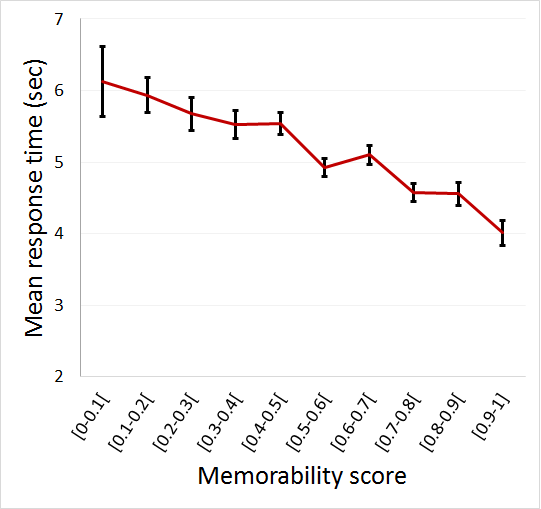
\includegraphics[width=0.45\columnwidth]{figures/Response_time_vs_Memorability.png}}
	\quad
	\caption{\label{fig:response_time_vs_memorability}(a) Distribution of the number of videos depending on memorability score ranges. (b) Mean response time for correct recognitions against memorability scores.}
\end{figure}
%(a) Sample of the dataset with key frames of videos sorted from most memorable (left) to less memorable (right).

Figure \ref{fig:response_time_vs_memorability} (b) shows that the response time to do a correct detection decreases when the memorability of the video increases.
We also observed a Pearson's correlation of $-0.36$ ($p<.0001$) between the response time on the targets and their memorability scores.
These two results indicate that participants tended to answer quicker when the videos were more memorable, even though the participants did not receive any instruction to do so.
This suggests that people tend to naturally answer rapidly after having recognized the video.
This also suggests either that the most memorable videos are also the most accessible in memory, and/or that the most memorable videos contain more early recognizable elements than the less memorable ones.
In \cite{shekhar_2017_show}, the response time of the participants was taken to be the measure of video memorability.
The authors chose this measure to avoid a long gap between viewing and recall stage.
Our results validate -- to some extent -- their modus operandi: the fact that the response time decreases linearly when the memorability increases suggest that the response time is a good indicator of the memorability of the videos (at least, in a recognition task). 
 %However, the linear continuous decrease in response time when memorability score values increase supports the first hypothesis: one can hardly imagine that the early recognizable elements (e.g., the face of a person, a particular place...) decreases linearly with the memorability of our 10-sec semantically consistent videos.
 %The hypothesis of a linear relation between the accessibility of the videos in memory and their memorability is consistent with the associative functioning of long-term memory \cite{tulving_1974_cue}.
 %Information stored in long-term memory is retrieved by way of association with other memories.
 %One can hypothesize that the memorability of a video depends on how interconnected with peoples' prior memory the memories of this video is: in our experiment, the most memorable videos would have been the most easily accessible in memory, thus the most rapidly retrieved.
%target vs. fillers
 %We observed no significant correlation ($r=-0.09, p=.276$) between the mean response time to do a false alarm and the memorability score of the sequence.
 %In conjunction with our previous hypothesis, only early recognizable elements could have played a role if we had observed such a correlation, not the accessibility in memory (because fillers are, by definition, videos that are not in memory).
 %Let us imagine that the videos' early recognizable elements explain alone that the most memorable videos are recognized quickly than the less memorable ones.
 %If we assume that recognizable elements are responsible of the false alarms by misleading the participants, we could have expected that early recognizable elements would have encouraged the participants to wrongly recognized fillers quickly when they were most memorable, since, as was suggested, people tend to naturally answer rapidly after having recognized the video.
 %But we observed no effect of early recognizable elements on response time for fillers, while we observed an effect of either this factor of accessibility in memory for targets, in the same conditions (outside of this factor).
 %This suggests that the presence of early recognizable elements does not explain the relation we observed between the response time and the memorability of the target videos, and thus that the hypothesis of the accessibility in memory is better.
%response time for correct recognitions vs. false alarms 
 %A Wilcoxon rank-sum test indicated that the response time was greater to do a correct recognition ($Mdn=4.5, \mu=4.88 sec$) than to do a false alarm ($Mdn=5.8, \mu=5.90 sec$), $Z=-5.10, p<.00001$.
 %One explanation is that participants tended to hesitate more before generating a false alarm than when correctly recognizing a target.
 %It points out the fact that memories of videos are generally not obvious but more blurred.
 %This is an interesting point to connect with the fact that human consistency is lower for typical than for neutral videos: because of the non obviousness of if they had memories or not, the part of subjectivity for typical videos could have fostered participants to answer when they hesitated if they were guessing that a video came from a movie they had seen or remembering it.
 %The higher degree of memorability of typical videos compare to the one for neutral videos could be partly due to this factor too.
 %Among other, this is also an argument in favour of the most "objective" possible measure to choose to constitute an extensive dataset for VM prediction.

%%%%%%%%%%%%%%%%%%%%%%%%%%%%%%%%%%%%%
\subsection{User context and memorability}%\cite{walker_1967_estimation}
To provide us with insights on which context-related factors collected through our questionnaire were linked to memorability, we processed to a logistic regression, using demographics and answers to the questionnaire as regressors, and the detection of a target video (with two possible discrete outcomes, detected or not) as observations to fit.
Regarding the participants' nationality, we grouped them into occidental (69 pers) and non-occidental (35 pers) categories, motivated by our use of occidental movies, which could have more meaning for occidental than for non-occidental people.
We also tested age and gender to reveal a potential bias in our movies' choice, that may be more memorable for people of a certain age and gender.
%The method provides a measure of the statistical significance of each feature in the model through their \textit{p}-value.
The model, in case of a single observation $n$, can be written as:
\begin{equation}
	y_{n}=
	\begin{cases}
	1 & \textit{if } \beta_0 + \sum\limits_{k=1}^K x_{n,k} \beta_k+\epsilon_n>0 \\
	0 & else
	\end{cases}
\end{equation}
where $y_{n}$ denotes the dependent variable which can take two values, 1 for recognition or 0 for omission of the $n$-th target observation, $x_{n,k}$ our k-th feature value (last view, number of views, nationality, age, gender), $\beta_{k}$ are the coefficients to be estimated, and $\epsilon_{n}$ indicates the error term.

%figure logistic regression (a), and movie last viewing and nb of viewing (b)
\begin{figure}[!htbp]
	\centering
	\subfloat[]{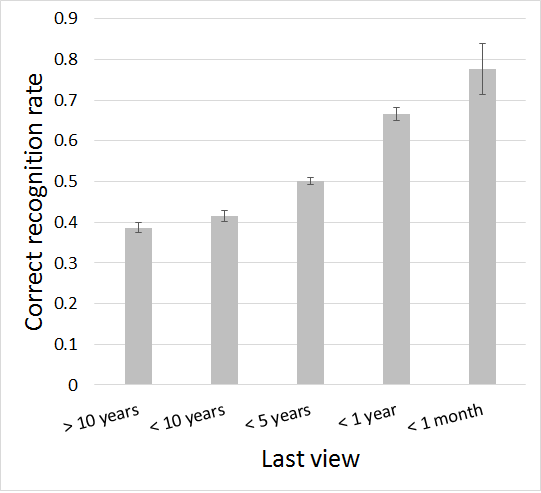
\includegraphics[width=0.45\columnwidth]{figures/film_last_viewing.png}}
	\quad
	\subfloat[]{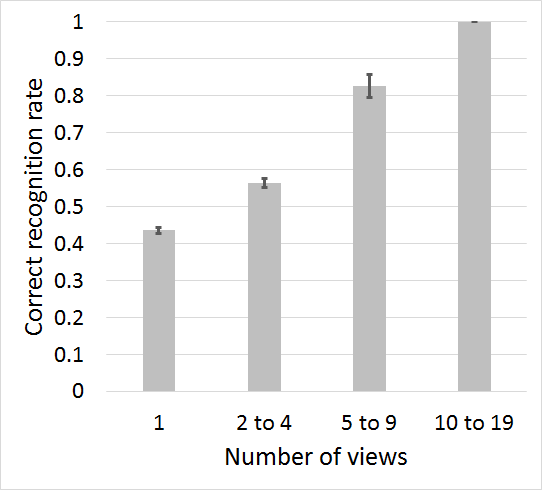
\includegraphics[width=0.45\columnwidth]{figures/nb_of_viewing.png}}
	\quad
	\caption{\label{fig:logistic_regression}Correct recognition rate depending on (a) when occurred the last viewing, and (b) the number of views.}
\end{figure}

%memorability change over time
According to the results of the logistic regression, the retention duration (last view) is highly negatively correlated with the probability to recognize a video ($\beta=-.37, p<.0001$).
Figure \ref{fig:logistic_regression} (a) shows that this decrease in memory for videos over time is continuous.
This result indicates that long-term memory of videos continues to be altered over time for years.
In the context or experiment, it implies that, to provide an accurate representation of an average long-term memory performance, a memorability score should correspond to a memory measure carried out as late as possible after the memorization.
%depends on the application and which type of memory is concerned.

%memorability and viewving repetition
The results of the logistic regression also show that the number of views is highly correlated with the probability to recognize a video ($\beta=.44, p<.0001$).
As expected, the more a movie was seen, the better the videos were memorized.
Figure \ref{fig:logistic_regression} (b) shows that this continues to be true even with more than 9 viewings (however, the number of observations -- 12 -- was very low for videos which belong to movies with 10 or more views).
One should note that the repetition of a viewing could not be the (only) factor involved in the above phenomenon; in particular, viewing again a movie may be the sign of a special interest which would explained a better memorization (e.g., via a greater attentional and emotional investment).
The fact remains that repetition is an important factor to ask people when measuring their prior memory.
Furthermore, a protocol used to build an extensive database for VM prediction should, in case of multiple measures of memory (e.g., after the memorization and then after a longer delay), avoid measuring twice the same items, because this repetition could artificially increase the performance measured for the last items.

%Ajouter Age et expliquer que les movies sont plutôt jeune génération -- donner corrélation Age*Memorability => pas possible
We observed no significant effects of the demographic factors (nationality, age and gender).
This suggests that the videos were equally susceptible to be recognized by the different participants (or, that the relations between these factors and the observations are too complex to have been captured by the model).

%%%%%%%%%%%%%%%%%%%%%%%%%%%%%%%%%%%%%
% Other results possible
%%%%%%%%%%%%%%%%%%%%%%%%%%%%%%%%%%%%%
%\subsection{Mean memorability of the videos compare to the movie they come from}
	%Corriger score par moyenne de mem du movie -- est-ce que ça a un sens ? Par le nombre de vue du movie ? par le moment où il a été vu?

%\subsection{Quality of the movies}
	%dvdrip vs. HD 720-1080 => Difference of memorability? => Interesting

%\subsection{movie genre and IMDB ratings}
	%test the momorability od the videos compare to the mean one of the movie.
	%Correct bu the mean participant's performance
	%And maybe other IMDB annotations/labels

%\subsection{Context}
	%Analyse the context (order of video presentation) influent the memo: to be check if we have enough information?
	%Une vidéo par rapport à toutes les autres différentes à un impact sur sa mem ?
	%S'inspirer de la technique de Bylinskii
	%tester la mémorability de séquences très proches (prise à intervalles très proche + vérif = même scène)

%\subsection{Features linked to memorability}
	%tester ces features comme dans 'What makes a photograph...'
	% Indoor/Outdoor, low-level visal feautures (color... -- i.e., as in isola et al.), salinecy maps

%\subsection{Indoor \textit{.vs} outdoor scenes}
	%indoor/outdoor comme isola et al. mais en contrecarrant l'effet de la couleur -- car ils expliquent que c'est par la corrrélation entre couleur et mémorabilité est expliqué par le fait que les couleurs plus froides sont d'exté.

%\subsection{Other points}
	%add other relevant points found in MIT papers e.g.,

%Corr Evolution of the memorability along time for videos scores
%Use order positions for that (e.g., mean memorability for position 1, 2... 120)


%%%%%%%%%%%%%%%%%%%%%%%%%%%%%%%%%%%%%
%\subsection{New manner to compute memorability scores: take into account time and FA}
%Une nouvelle manière pour prendre en compte les FA dans les scores de mémorabilité applicable à l'étude de la mémorabilité sur les images
%Ce qui à la fin de cette section vient avant permet de conclure cette partie en disant : la meilleure façon de calculer les scores de mémorabilité, c'est comme ça.
% The question here is: "Must we correct our memorabiliy scores by taking into account the mean memorability of the participants --> No, of the movie --> No' --> So the point here is just to provide an overview.

%%%%%%%%%%%%%%%%%%%%%%%%%%%%%%%%%%%%%%%%%%%%%%%%%%%%%%%%%%%%%%%%%%%%%%%%%%%%%%%%%%%%%%%%%%%%%%%%%%%%%%%%%%%%%%%%%%%%%%%%%%%%%%%%%%%%%%%%%%%%%%%%%%%%%%%%%
\section{Memorability prediction} %for Khartik
\label{mem-pred}
%%%%%%%%%%%%%%%%%%%%%%%%%%%%%%%%%%%%%%%%%%%%%%%%%%%%%%%%%%%%%%%%%%%%%%%%%%%%%%%%%%%%%%%%%%%%%%%%%%%%%%%%%%%%%%%%%%%%%%%%%%%%%%%%%%%%%%%%%%%%%%%%%%%%%%%%%
Until now, we have presented the video collection and the annotation protocol together with some insights on human VM. 
%We then computed memorability scores and analyzed how different users fared in remembering the video sequences from the movies they have already watched.
In this section, we move towards building a machine learning model that can learn and then predict the VM score of a video from its audio-visual features.
The main goal of modelling is to understand if VM is predictable, and if yes identify which features: generic, perceptual, or semantic, are suitable for such prediction.
We pose the problem as a standard regression problem and Figure \ref{prop-apprch} illustrates different steps in our method.
%First, we see that the videos are converted into feature vectors and then a regression model is trained that can in-turn predict the memorability scores for new videos.
In the following sub-sections, we explain our choice of features and models to address the problem in hand.

\begin{figure}[h]	  
	\centering
	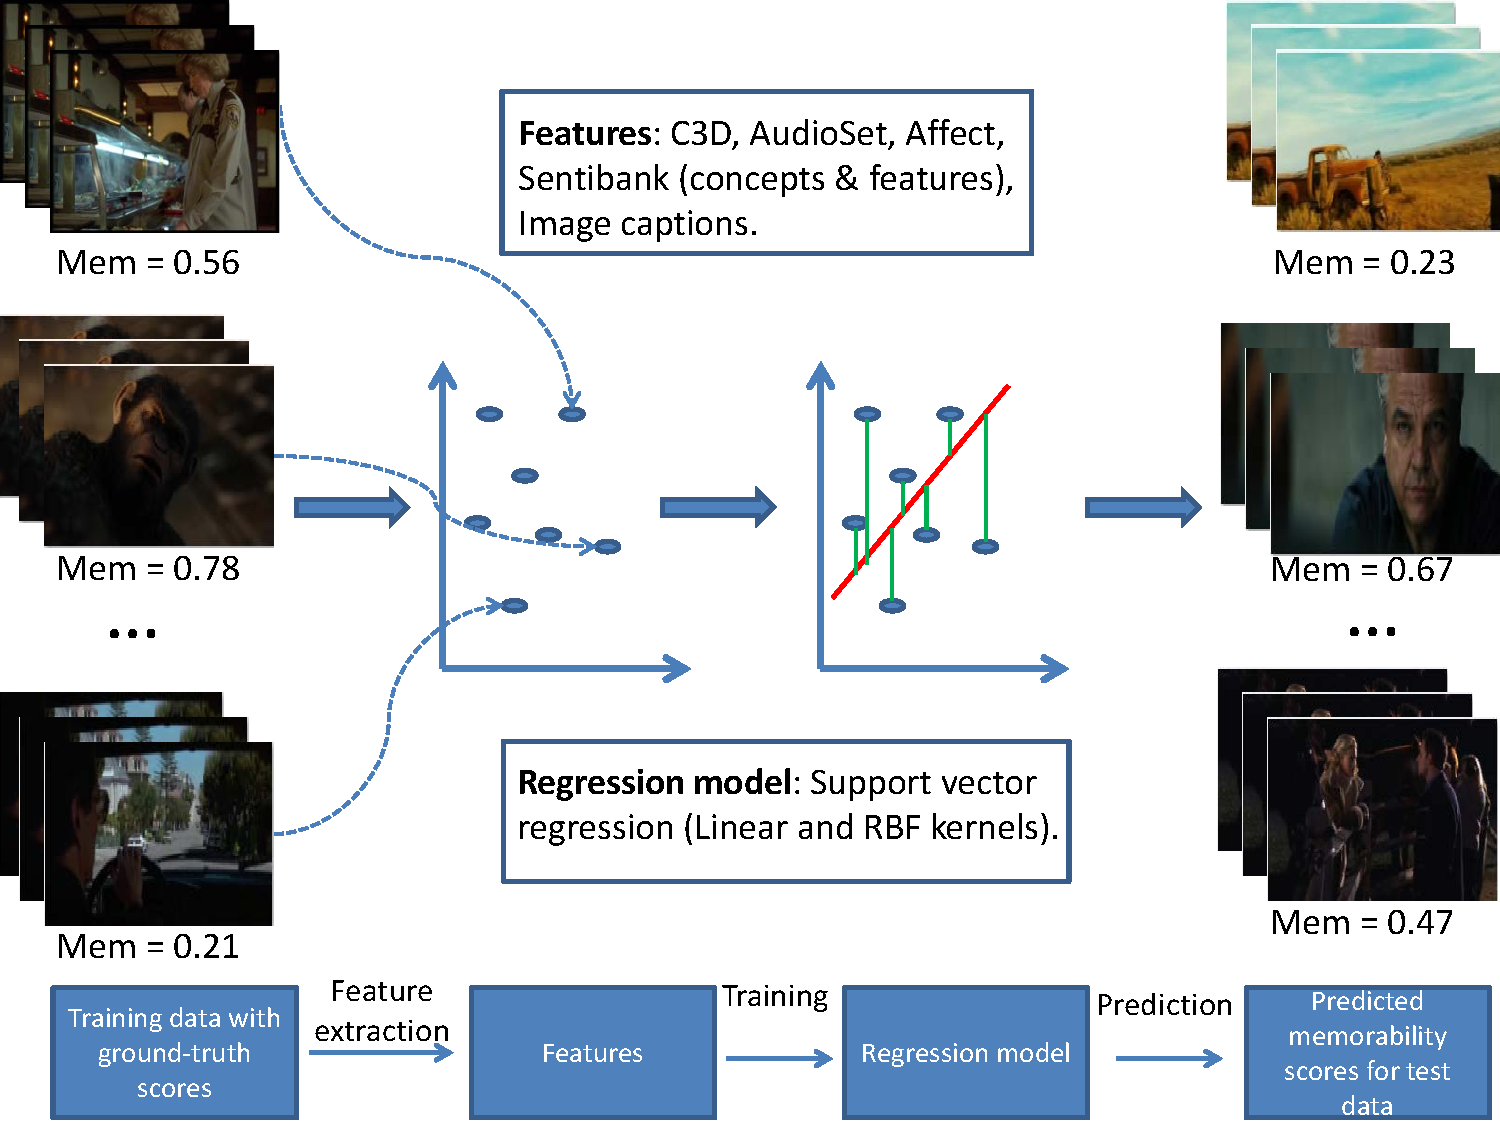
\includegraphics[width=0.9\columnwidth]{figures/approach.pdf}
	\caption{Proposed approach for memorability score prediction.}
	\label{prop-apprch}
\end{figure}

%Before we go into the technical details about the different audio-visual features and regression models we explored, we will talk about how we split our dataset.
To build our predictive model, we split the dataset, at the level of movies, into training (70\%), validation (15\%) and test (15\%) data, which translates into 70 movies in the training set and 15 movies each in the validation and test sets.
We chose to split our dataset at the level of movies, instead of the videos, in order to avoid videos from the same movie being present in the training as well as the evaluation (validation+test) set. To ensure that such random split did not lead to any mismatch, we computed the average number of annotations per video in each of them. 
We observe that the numbers of annotations are balanced: each video in the test set has around 10 annotations while there are 9 annotations for each one in the train set on an average.

\subsection{Feature extraction}
\label{feat-extr}
%We explore a variety of audio-visual features in building a model that can predict memorability scores for new videos.
The task of remembering a specific video has a high cognitive complexity in general, suggesting that it requires a semantic understanding of the content and/or some other perceptual factors such as the emotion conveyed by the video. 
Many users who participated in our experiments indicated that it is a difficult task.
While trying to build a machine learning model for such a task, we explore different kinds of features that can be extracted from the audio-visual signal.
We investigate a variety of generic state-of-the-art features (\cite{c3d-feat}, \cite{audioset-feat}) and compare them with other semantic (\cite{caption-feat}) and perceptual (emotion) features (\cite{sb-feat}).

%We mostly stick to state-of-the-art deep learning features that have been proposed in vision and audio research communities for tasks like video classification \cite{c3d-feat}, event detection \cite{audioset-feat}, image captioning \cite{caption-feat}, and concept detection \cite{sb-feat}. 

\subsubsection{Spatio-temporal visual features (C3D)}
\label{c3d-feat}
These features are extracted from the C3D model, a 3-dimensional convolutional network proposed for generic video analysis \cite{c3d-feat}. 
The main motivation to use C3D is that it encodes both the spatial and temporal information in the video.
The model has been proposed for video analysis and is not an extension of a model for image analysis, unlike other state-of-the-art models like VGG16 \cite{vgg16}.
We use the publicly available model trained on the Sports-1M dataset \cite{c3d-feat} and extract the output of the fully connected layer -- fc6 of the network with a dimensionality of 4096.
We additionally explore the use of principal component analysis (PCA) (named C3D (PCA) in Table \ref{res-4-10-ann}) for the dimension reduction, as the original dimensionality is very high when compared to other features.

\subsubsection{Audio features (AudioSet)}
\label{as-feat}
Using a recently released AudioSet \cite{audioset-feat} model, which was trained on a large dataset for event detection, we extract 128-dimensional embeddings for each audio track associated with a video in our dataset.
We use these embeddings for training the regression models.
The motivation to use these features is that they are state-of-the-art in the audio event detection research and events could play a major role in how people remember sequences in movies.
Additionally, we wanted to investigate how the audio channel contributes to building a model for VM prediction.

\subsubsection{Emotion related features (SentiBank and Affect)}
\label{emo-feat}
As research in psychology showed that emotion and memory are correlated \cite{emo-mem}, we investigate the use of emotion-related feature in our prediction system.
For modelling emotion from the visual content, we resort to a visual sentiment concept detector: SentiBank \cite{sb-feat}.
SentiBank is a set of 1200 trained visual concept detectors providing a mid-level representation of sentiment from visual content.
We use the binary code for concept detection, from images, provided by the authors.
The SentiBank concept detector provides two pieces of information: concepts with probabilities and features.
Concepts are adjective--noun pairs and the probability represents how likely each concept is depicted visually in an image.
Examples of some concepts in the SentiBank ontology are: \emph{young driver}, \emph{scary face}, \emph{terrible pain}, etc.

We sample one frame for every second of the video in our dataset, resulting in 10 frames per video.
We run the SentiBank concept detector on each of these 10 frames and rank the concepts based on the probability of their occurrence in the frame and take the top-50 concepts.
We extract 300-dimensional word embeddings (Word2Vec \cite{word2vec}), for each of the 50 concepts and take an average to obtain a single vector per frame.
We repeat this process for all the 10 frames and take the average of all the vectors to obtain a single feature vector for each video.
Sentibank detectors also provide a 4096-dimensional feature for each frame and we take the average across all the frames to obtain one 4096-dimensional feature vector for each video.
In the end, we use a 300-dimensional concept vector and a 4096-dimensional feature vector.

In addition to SentiBank concepts, we investigate other ways to capture emotional content in a video. 
Following a circumplex model of affect (the experience of emotion) \cite{affect-model}, we define arousal as the dimension of affect that measures the excitement in the video, while valence measures whether the video invokes positive or negative emotion.
We resort to an audio-visual analysis of the video to obtain its arousal and valence scores using the method described in \cite{affect}.
For each frame in the video, we compute the arousal and valence scores using the method proposed in \cite{affect}.
In order to keep a fixed dimensionality of the feature vector, we take the first 200 frames in the video because of the varying frame rates across the videos.
We concatenate the arousal and valence scores for the first 200 frames in each video resulting in a 400-dimensional feature vector (200 for arousal and 200 for valence) for a video.

\subsubsection{Visual semantic features (Image captions)}
\label{sem-feat}
Visual semantics are known to play an important role in image memorability (\cite{sem-mem}, \cite{squalli_2017_deep}).
We utilize the state-of-the-art research in image captioning to capture such high-level semantics of the video \cite{caption-feat}.
We sample one frame for every second of the video in our dataset, resulting in 10 frames per video.
For each of these 10 frames, we run the caption detector (code provided by the authors) and obtain a caption for the frame.
For each non-functional word in the caption, we extract 300-dimensional word embeddings (Word2Vec \cite{word2vec}) and take an average across all the words to obtain a single vector per frame.
We repeat this process for all the 10 frames and take the average of all the vectors to obtain a single 300-dimensional feature vector for each video.

\subsection{Modelling and evaluation metric}
\label{model-eval}
We use the features discussed in Section \ref{feat-extr} to train a Support Vector Regression (SVR) model for the VM score prediction. The choice of SVR is guided by the nature of the problem as well as by the small size of the dataset. We have chosen to go with the same regressor for all the features because our focus is mainly on identifying which features are more important for VM prediction. This way we ensure that the difference in performances is because of the features themselves. Note that, in addition to the variety of features explained in Section \ref{feat-extr}, we also explore a combination of all the features by concatenating them into a single feature vector.
While performing such a concatenation, we use the low-dimension version of the features for C3D and SentiBank features, obtained after applying a dimension reduction method (PCA) to the original set. In the experiments where we use PCA for C3D and SentiBank features, we retain 95\% of variance in the data while reducing the feature dimensions. 

We use the grid search strategy to obtain the best hyper-parameters for SVR in term of the Mean Squared Error ($MSE$) between the predicted scores and the ground-truth on the validation set. The choice of hyper-parameters in the grid search are: kernel = $\{$linear, RBF$\}$, $C$ = $\{0.1, 1, 10, 100, 1000\}$ and $\gamma$ = $\{0.01, 0.1, 1, 10, 100\}$.

%Since we are posing the memorability prediction problem as a regression problem, we use the standard regression metric: Mean squared error ($MSE$) for evaluation.
The prediction performance is evaluated by the Spearman correlation ($SpCorr$), which measures the rank correlation between the predicted memorability scores and the ground-truth scores. This metric is chosen as (1) we focus more on the relative memorability between videos rather than on  their absolute memorability scores, and (2) it gives an indication of how close the predicted memorability scores are to the human consistency when annotating memorability scores.


%Each of the videos in our dataset has multiple annotations and we pick sequences with at least 4 annotations for training the models.
%In this way, we eliminate movies that were not seen by a majority of the users who participated in our experiment.
%Since we are using an SVR with linear and rbf kernels, we train the models on the training set (70 movies) and validate the model on the validation set (15 movies), before reporting the final scores on the test set (15 movies).
%We pick the SVR model parameters: kernel (linear or RBF), $C$ and $\gamma$ that give the best performance on the validation set.
%We retrain the model with these parameters using the training set and evaluate on the final test set.
%In the experiments where we use a dimension reduction method (PCA) for C3D and SentiBank features, we retain 95\% of variance in the data while reducing the feature dimensions. 

\begin{figure}[h]	  
	\centering
%	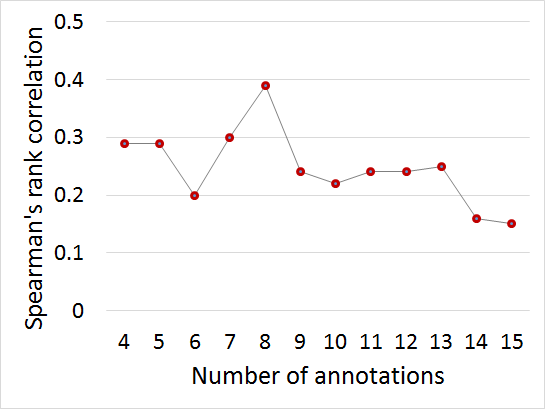
\includegraphics[width=0.7\columnwidth]{figures/annotations_modelling.png}
	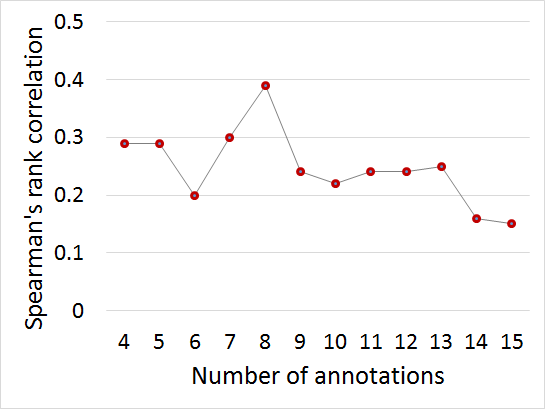
\includegraphics[width=0.7\columnwidth]{figures/annotations_modelling.png}
	\caption{Spearman correlation on the validation set with models using image captioning features trained on videos with varying number of annotations.}
	\label{num-ann}
\end{figure}

\begin{table*}
	\centering
	\renewcommand{\arraystretch}{1.2}
	\begin{tabular}{|c|c|c|c|c|c|c|}
		\hline
		\textbf{Feature} & \textbf{Feature type}& \textbf{Dimension}& \multicolumn{2}{c|}{\textbf{$SpCorr$($\geq$ 4 annotations)}} & \multicolumn{2}{c|}{\textbf{$SpCorr$ ($\geq$ 8 annotations)}}\\
		% \hline
		% \textbf{Inactive Modes} & \textbf{Description}\\
		\cline{4-7}
		& & & \emph{validation set}& \emph{test set} & \emph{validation set}& \emph{test set}\\ \hline
		C3D& visual spatio-temporal& 4096& 0.20& 0.26& 0.31& 0.34\\ \hline
		C3D (PCA)& visual spatio-temporal & 225& 0.24& 0.21& 0.18& 0.17\\ \hline
		AudioSet& audio related& 128& 0.23& 0.22& 0.21& 0.24\\ \hline
		Affect& affect related& 400& 0.19& 0.17& 0.26& 0.23\\ \hline
		SentiBank concepts& emotion related& 300& 0.16& 0.13& 0.15& 0.17\\ \hline
		SentiBank features& emotion related& 4096& 0.25& 0.21& 0.27& 0.26\\ \hline
		SentiBank features (PCA)& emotion related & 225& 0.22& 0.21& 0.22& 0.23\\ \hline
		Captions& visual semantics & 300& \textbf{0.29}& \textbf{0.31}& \textbf{0.39}& \textbf{0.38} \\ \hline
		Combination (PCA)& combine all features & 1578& 0.24& 0.23& 0.29& 0.27\\ \hline		
	\end{tabular}
	\caption{Prediction results in terms of Spearman correlation scores on validation and test data for different features with models trained on videos that have at least 4 (columns 4-5) or 8 (columns 6-7) annotations.}
	\label{res-4-10-ann}	
\end{table*}

\subsection{Memorability prediction results}
\label{pred-res}
In this section, we will discuss how the models trained on different features perform while predicting memorability scores of new videos.
%We report the results of the prediction on both the validation and test sets.
%We also report only correlation scores: $SpCorr$ and not $MSE$ keeping in mind the space constraints.
%Additionally, $SpCorr$ is more informative because it provides a rank correlation between the predicted memorability scores and the ground truth.
%We compute the average number of annotations per video in the train and test set for both the cases ($\geq$ 4 and $\geq$ 8 annotations).
%We observe that the number of annotations in the train and test sets are balanced and there is no mismatch.
%For example, each sequence in the test set has around 10 annotations while there are 9 annotations for each sequence in the training on an average.
Table \ref{res-4-10-ann} reports the prediction results obtained by the SVR model when trained on different features, for the validation and test sets.
Two sets of results are reported: $SpCorr$ ($\geq$ 4 annotations) and $SpCorr$ ($\geq$ 8 annotations). The former 
corresponds to the prediction capability of the model when trained on videos with at least 4 annotations, and the latter corresponds to the results when trained on videos with at least 8 annotations where the ground-truth is better annotated.
%We will further discuss why we report the results with the model trained on videos with at least 8 annotations.

As it can be seen, visual semantic features derived from image captioning clearly offer better prediction results compared to all other considered features. This is not surprising as they capture visual attributes along the scene, which are known to play an important role in human memory. This is also inline with a previous study in IM \cite{squalli_2017_deep} where image captioning-based features helped better predict IM than the conventional CNN features. %These best prediction results (i.e., 0.31 and 0.38 for the test sets) are quite close to the human consistency shown in Figure \ref{fig:human_consistency}b (i.e. about 0.36 when having 4 annotations per video and about 0.47 when having 8 annotations per video).
When predicting VM on the test set, C3D features showed to be quite effective to the task as they encode the visual spatio-temporal information of the video. On the contrary, audio information captured by AudioSet features does not seem to be enough for VM prediction. One of our initial hypotheses was that emotion would play an important role in VM, supported by literature from psychology \cite{emo-mem}.
However, when observing the results in Table \ref{res-4-10-ann}, both Affect \cite{affect} and SentiBank \cite{sb-feat} performed quite poorly compared to the image captioning features.
%Observing the first set of results in Table \ref{res-4-10-ann}, where we have at least 4 annotations per video, we can clearly see that the image captions and C3D occupy the top-2 places in terms of performance on the test set. 
%Image captions capture the visual semantics in the video, while C3D features encode the visual spatio-temporal information.
%These results are consistent with previous results on predicting image memorability \cite{squalli_2017_deep}.
%Our dataset consists of videos taken from movies that have a specific story-line; semantics and spatio-temporal information seem to be playing an important role in people remembering specific scenes from movies.
%Other features like AudioSet come close to the performance of the C3D, but only audio signal does not seem to be enough for predicting video memorability.
Another observation from Table \ref{res-4-10-ann} is that the combination of all the features (last row in the table) does not appear in the top-3 best performing features. One of the reasons for this could be that there is a lot of redundance when combining all the features into a single feature vector, or it could be that the size of the combined feature vector is too big when compared to the size of the dataset. Thus, in future work we could look at selectively combining the features to investigate if that improves the performance. 

%One of our initial hypotheses was that emotion would play an important role in VM, supported by literature from psychology \cite{emo-mem}.
%Please recall that we used different set of features to encode the emotion in a video: Affect \cite{affect} and SentiBank \cite{sb-feat}.
%However, when observing the results in Table \ref{res-4-10-ann}, both Affect \cite{affect} and SentiBank \cite{sb-feat} performed quite poorly compared to the image captioning.
%we can say that the SentiBank features (fourth row from bottom) perform slightly better than the affect features (sixth row from bottom).
%But the models trained on image captioning features clearly out-perform those trained on emotion features.
%This could be because of the following reasons: our choice of features to capture emotion related information is not suitable for the task, or the performance of the emotion prediction models is not good enough for memorability prediction, or we are unable to establish the correlation between emotion and memorability because of the limited size of our dataset.
%From the analysis on this dataset and the features we used for capturing emotion related information, we \emph{cannot} conclude that emotion plays an important role in memorability.
%In the future, we could investigate more robust emotion/affect prediction models to confirm that both emotion and memorability are correlated as suggested in the literature \cite{emo-mem}.

As our dataset contains videos with different numbers of annotations, we further investigate the effect of the number of annotations on the prediction performance.
%Based on our experimental results, we observe that the image captioning feature performs the best while using training videos that have at least 4 annotations.
%For this purpose, we train different SVR models with varying number of annotations on the training set using image captioning features only.
For this purpose, we train a first SVR model, using image captioning features, on videos with at least 4 annotations and use this model to predict the memorability score for videos in the validation set.
We repeat this process for different numbers of annotations per video (from 4 to 15) in the training set.
Please note that the validation set in each of the repetitions is fixed and only the training set changes.
We provide a demonstration of how $SpCorr$ varies with an increasing number of annotations in the training set in Figure \ref{num-ann}.
As can be seen, $SpCorr$ first increases up to 5 annotations and then remains more or less constant before decreasing (beyond 10 annotations).
In the wake of this observation, we also investigated the performance of all the features when we train the regression model with videos that have at least 8 annotations as reported in the second part of Table \ref{res-4-10-ann}: $SpCorr$ ( $\geq$ 8 annotations).

Comparing the two sets of results in Table \ref{res-4-10-ann}, we observe that globally the models trained on videos with at least 8 annotations perform better than the models trained on videos with at least 4 annotations.
These results are comparable to the human consistency analysis shown in Section \ref{ssec:human}.
%We can say that with an increase in the number of annotations per video, we can expect an increase in the performance until a certain number of annotations (8 annotations in this case).
%From the table, we also observe that the scores for validation set and test set are very similar across the two sets of results.
We finally performed an additional 10-fold cross-validation on videos with at least 8 annotations (train+validation set) using the image captioning features. From this study, we re-confirmed that there is no overfitting issue in our model and we observed the average value of $SpCorr$ across the 10 folds to be 0.33, which is close to the performance on the test set.
%Looking at the performance in the cross-validation experiment, we can say that there is no over-fitting because of the small dataset.

%%%%%%%%%%%%%%%%%%%%%%%%%%%%%%%%%%%%%%%%%%%%%%%%%%%%%%%%%%%%%%%%%%%%%%%%%%%%%%%%%%%%%%%%%%%%%%%%%%%%%%%%%%%%%%%%%%%%%%%%%%%%%%%%%%%%%%%%%%%%%%%%%%%%%%%%%
\section{Conclusions}
\label{conclusions}
%%%%%%%%%%%%%%%%%%%%%%%%%%%%%%%%%%%%%%%%%%%%%%%%%%%%%%%%%%%%%%%%%%%%%%%%%%%%%%%%%%%%%%%%%%%%%%%%%%%%%%%%%%%%%%%%%%%%%%%%%%%%%%%%%%%%%%%%%%%%%%%%%%%%%%%%%
%protocol
In this paper, we have presented a novel protocol to collect long-term memorability annotations for videos, which enabled us to build an important dataset to support research in this subject. We then performed a range of statistical studies on this dataset to understand important factors in the annotation process as well as how they can affect the video memorability. One of our key observations is that high human consistency in video memorability can be obtained by only about 18 annotations, which is significantly lower than for images according to the previous studies. We finally proposed computational models for video memorability prediction where we investigated the use of various audio-visual features for the task. For this, we observed that the visual semantic features offer the best prediction result, which re-confirms the correlation between the visual attributes and memorability. Our current work focuses on building a large scale video memorability dataset using crowdsourcing annotations.  

%and built a dataset publicly available.
%We measured memory performance after weeks to years.
%It appears from the analysis that memory of videos continues to decrease for years, which justifies a measurement of memory performance after a significant retention duration, longer than what is proposed in previous work.
%The principal weakness of our protocol is the part of subjectivity susceptible to enter in our measure of memorability, that one should counteract by appropriate controls.
%Our current work focuses on collecting VM annotations at a large scale using crowdsourcing, measuring VM in a more objective manner.

%modelling Karthik
%After exploring a variety of generic (C3D, AudioSet), perceptual (SentiBank, Affect), and semantic (Image captions) features, we can say that a model trained with  semantic features provides predictions that are most correlated with ground truth memorability scores.
%It might be very interesting to investigate if these findings hold for generic video types other than movies.
%Future research could involve investigating the memorability prediction performance on other generic videos using the existing set of features as well as other important features.
%We also found that emotion features are not that well correlated with ground truth memorability scores, as indicated in psychology literature.

%An immediate direction for future research would be to explore other approaches to encode emotion in videos and investigate whether we can improve the prediction performance using these approaches.
%We also investigated the number of annotations required to train a model and found a sweet spot where the performance is optimal.
%%%%%%%%%%%%%%%%%%%%%%%%%%%%%%%%%%%%%%%%%%%%%%%%%%%%%%%%%%%%%%%%%%%%%%%%%%%%%%%%%%%%%%%%%%%%%%%%%%%%%%%%%%%%%%%%%%%%%%%%%%%%%%%%%%%%%%%%%%%%%%%%%%%%%%%%%
%\addtolength{\textheight}{-12cm}   % This command serves to balance the column lengths
                                  % on the last page of the document manually. It shortens
                                  % the textheight of the last page by a suitable amount.
                                  % This command does not take effect until the next page
                                  % so it should come on the page before the last. Make
                                  % sure that you do not shorten the textheight too much.
%%%%%%%%%%%%%%%%%%%%%%%%%%%%%%%%%%%%%%%%%%%%%%%%%%%%%%%%%%%%%%%%%%%%%%%%%%%%%%%%%%%%%%%%%%%%%%%%%%%%%%%%%%%%%%%%%%%%%%%%%%%%%%%%%%%%%%%%%%%%%%%%%%%%%%%%%
%\section*{Appendix}
%%%%%%%%%%%%%%%%%%%%%%%%%%%%%%%%%%%%%%%%%%%%%%%%%%%%%%%%%%%%%%%%%%%%%%%%%%%%%%%%%%%%%%%%%%%%%%%%%%%%%%%%%%%%%%%%%%%%%%%%%%%%%%%%%%%%%%%%%%%%%%%%%%%%%%%%%
 %Liste des features (comme/ceux de MediaEval 2015 à donner au téléchargement avec le début en sec de nos sequences)
 %Release text file for movie title, start/end time + features

%%%%%%%%%%%%%%%%%%%%%%%%%%%%%%%%%%%%%%%%%%%%%%%%%%%%%%%%%%%%%%%%%%%%%%%%%%%%%%%%%%%%%%%%%%%%%%%%%%%%%%%%%%%%%%%%%%%%%%%%%%%%%%%%%%%%%%%%%%%%%%%%%%%%%%%%%
%\section*{Acknowledgment}
%%%%%%%%%%%%%%%%%%%%%%%%%%%%%%%%%%%%%%%%%%%%%%%%%%%%%%%%%%%%%%%%%%%%%%%%%%%%%%%%%%%%%%%%%%%%%%%%%%%%%%%%%%%%%%%%%%%%%%%%%%%%%%%%%%%%%%%%%%%%%%%%%%%%%%%%%
%optional (%to acknowledge grants, funding, editing assistance and what have you.)

%%%%%%%%%%%%%%%%%%%%%%%%%%%%%%%%%%%%%%%%%%%%%%%%%%%%%%%%%%%%%%%%%%%%%%%%%%%%%%%%%%%%%%%%%%%%%%%%%%%%%%%%%%%%%%%%%%%%%%%%%%%%%%%%%%%%%%%%%%%%%%%%%%%%%%%%%
%% BIBLIOGRAPHY
%%%%%%%%%%%%%%%%%%%%%%%%%%%%%%%%%%%%%%%%%%%%%%%%%%%%%%%%%%%%%%%%%%%%%%%%%%%%%%%%%%%%%%%%%%%%%%%%%%%%%%%%%%%%%%%%%%%%%%%%%%%%%%%%%%%%%%%%%%%%%%%%%%%%%%%%%
\bibliographystyle{ACM-Reference-Format}
\bibliography{references} 
%%%%%%%%%%%%%%%%%%%%%%%%%%%%%%%%%%%%%%%%%%%%%%%%%%%%%%%%%%%%%%%%%%%%%%%%%%%%%%%%%%%%%%%%%%%%%%%%%%%%%%%%%%%%%%%%%%%%%%%%%%%%%%%%%%%%%%%%%%%%%%%%%%%%%%%%%
\end{document}